\documentclass[a4paper, 11pt]{article}

\usepackage[T2A]{fontenc}
\usepackage[utf8]{inputenc}
\usepackage[english, russian]{babel}
\usepackage[top=2cm, bottom=2cm, right=2cm, left=2cm]{geometry}
\usepackage{amsmath}
\usepackage{graphicx}
\usepackage{subcaption}
\usepackage{float}
\usepackage{tabularx}

\usepackage{amsmath,booktabs}
\usepackage{array}

\usepackage{tabu}
\newcommand\tline[2]{$\underset{\text{#1}}{\text{\underline{\hspace{#2}}}}$}
%Change label separator
\usepackage{caption}
\captionsetup[table]{labelformat=simple, labelsep = endash}
\captionsetup[figure]{labelformat=simple, labelsep = endash}

\usepackage{indentfirst}


\begin{document}
	\parindent=1.27cm
	\begin{titlepage}
		\centering
		{\fontsize{12pt}{5cm}\selectfont \bfseries Министерство образования и науки Российской Федерации} \\ \vspace{0.5cm}
		{\fontsize{7pt}{5cm}\selectfont ФЕДЕРАЛЬНОЕ ГОСУДАРСТВЕННОЕ АВТОНОМНОЕ ОБРАЗОВАТЕЛЬНОЕ УЧРЕЖДЕНИЕ ВЫСШЕГО ПРОФЕССИОНАЛЬНОГО ОБРАЗОВАНИЯ} \\ 
		\vspace{1cm}
		{\fontsize{12pt}{5cm}\selectfont \bfseries САНКТ-ПЕТЕРБУРГСКИЙ УНИВЕРСИТЕТ ИНФОРМАЦИОННЫХ ТЕХНОЛОГИЙ, МЕХАНИКИ И ОПТИКИ} \\ \vspace{1.5cm}

		{\fontsize{14pt}{5cm}\selectfont Кафедра \hspace{1cm} \underline{Систем Управления и Информатики}  \hspace{1cm} Группа \underline{Р3340}} \\ 
		\vspace{2cm}

		{\fontsize{20pt}{5cm}\selectfont \bfseries Лабораторная работа №8} \\
		{\fontsize{12pt}{5cm}\selectfont \bfseries “ЭКСПЕРИМЕНТАЛЬНОЕ ПОСТРОЕНИЕ ОБЛАСТЕЙ
			УСТОЙЧИВОСТИ ЛИНЕЙНОЙ СИСТЕМЫ НА ПЛОСКОСТИ
			ДВУХ ПАРАМЕТРОВ
			”} \\
		{\fontsize{14pt}{5cm}\selectfont Вариант - 11} \\
		\vspace{1.5cm}

		\flushleft

		{Выполнил \hspace{2cm} \tline{(фамилия, и.о.)}{9cm} (подпись)} \\
		\vspace{2cm}

		{Проверил \hspace{2cm} \tline{(фамилия, и.о.)}{9cm} (подпись)} \\
		\vspace{5cm}

		"\underline{\hspace{0.7cm}}"\hspace{0.2cm}\underline{\hspace{2cm}}\hspace{0.2cm}20\underline{\hspace{0.7cm}}г. \hspace{2cm} Санкт-Петербург, \hspace{2cm} 20\underline{\hspace{0.7cm}}г. \\ \vspace{1cm}

		Работа выполнена с оценкой \hspace{1cm} \underline{\hspace{8cm}} \\ 
		\vspace{1cm}
		Дата защиты "\underline{\hspace{0.7cm}}"\hspace{0.2cm}\underline{\hspace{2cm}}\hspace{0.2cm}20\underline{\hspace{0.7cm}}г.

	\end{titlepage}


\paragraph{Цель работы: }Ознакомление с экспериментальными методами построения областей устойчивости линейных динамических систем и изучение влияния на устойчивость системы ее параметров.
\paragraph{Исходные данные.} Необходимо исследовать систему при $g = 0$, $y(0) = 1$ и $T_1 = 3$. Сама система представлена на следующем рисунке.


\begin{figure}[h]
	
	\center{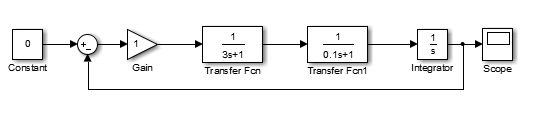
\includegraphics[width=0.7\linewidth]{0.png}}
	\\
	\centering Рисунок 1 - Схема моделирования
	
\end{figure}
\section{Устойчивость системы}

\begin{figure}[h]

	\center{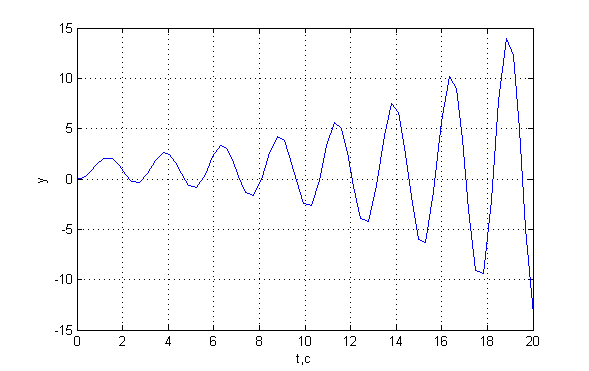
\includegraphics[width=0.7\linewidth]{1}}
	\\
		\centering Рисунок 2 - Графика неустойчивости САУ
\end{figure}

\begin{figure}[h]
	
	\center{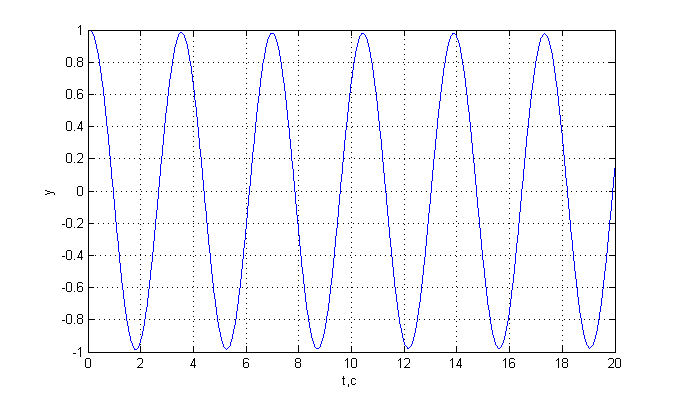
\includegraphics[width=0.7\linewidth]{2}}
	\\
	\centering Рисунок 3 - Граница устойчивости колебательного типа.
\end{figure}

\begin{center}
	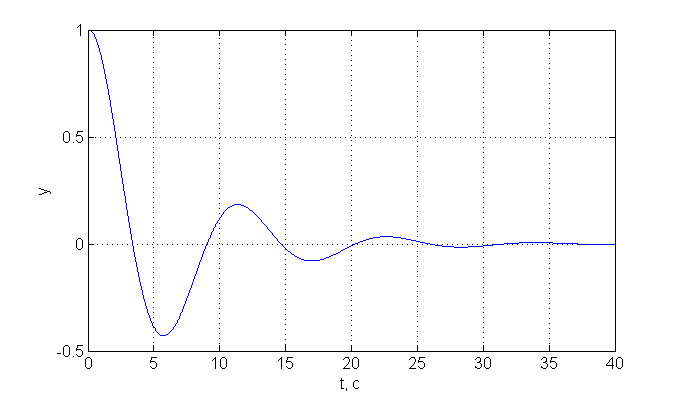
\includegraphics[width=0.7\linewidth]{3}
	\\
\centering Рисунок 4 - Графика устойчивости САУ
	

\end{center}

\begin{center}
	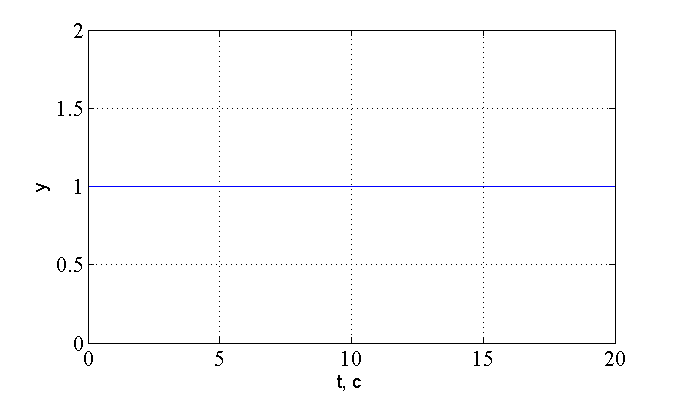
\includegraphics[width=0.7\linewidth]{5}
	\\
	\centering Рисунок 5 - Граница устойчивости нейтрального типа
	
	
\end{center}

\newpage
\section{Анализ устойчивости системы}
\subsection{Построим экспериментальную границу устойчивости}

\begin{table} [h!]
	\centering
	\caption{Экспериментальные данные.}
	\tabulinesep = 2mm
	\begin{tabu} spread 1em{|c|c|c|c|c|c|c|c|c|c|c|c|}
		\hline
		$T_2$ & 0.1 & 0.5 & 1 & 1.5 & 2 & 2.5 & 3 & 3.5 & 4 & 4.5 & 5 \\  \hline
		$k$ & 10.3 & 2.3 & 1.3 & 1 & 0.83 & 0.73 & 0.67 & 0.62 & 0.58 & 0.55 & 0.53  \rule{0pt}{5pt} \\ 
		\hline
	\end{tabu}
\end{table}

\subsection{Теоретический расчет границы устойчивости с использованием критерия Гурвица}


    Передаточная функция 
    \begin{equation}
      W(s) = \frac{K}{T_1 T_2 s^3 + (T_1 + T_2)s^2 + s + K}
    \end{equation}


Для анализа устойчивости системы составим матрицу Гурвица.
\begin{equation}
A = \begin{bmatrix}
3 + T_2 &  k & 0 \\
3 T_2 & 1 & 0 \\
0 & 3 + T_2 & 1
\end{bmatrix}
\end{equation}

САУ устойчивость на границе когда % MathType!MTEF!2!1!+-
\begin{equation}
\begin{cases}
3 + T_2 - k 3 T_2 = 0 \\
3 + T_2 > 0 \\
K > 0
\end{cases}
\end{equation}

\begin{equation}
k =\frac{3 + T_2}{3T_2}
\end{equation}

\begin{center}
		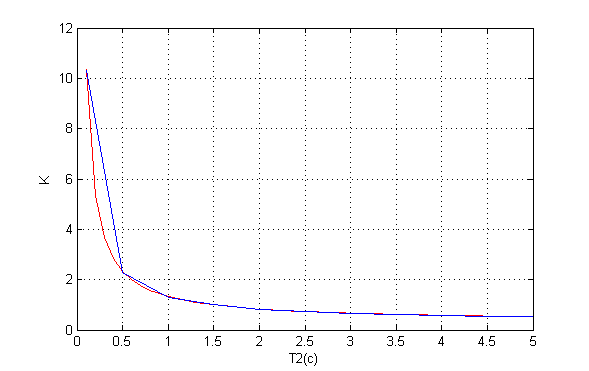
\includegraphics[width=0.7\linewidth]{4}
		\\
	\centering  Рисунок 6 - Графика границы устойчивости САУ

	
\end{center}

\newpage
\section*{Выводы}
При проектировании систем большое значение имеет определение областей устойчивости в плоскости реальных параметров, присущих системе. Аналитическую оценку позволил получить критерий Гурциа. Соотвественно по составленной матрице (2) мы смогли получить и составить условия границы устойчивоси (3) и (4). Система является устойчивой ,соответственно, множество значений параметров находится ниже границы устойчивости (при % MathType!MTEF!2!1!+-
% feaagGart1ev2aaatCvAUfeBSjuyZL2yd9gzLbvyNv2CaerbuLwBLn
% hiov2DGi1BTfMBaeXatLxBI9gBaerbd9wDYLwzYbItLDharqqtubsr
% 4rNCHbGeaGqiVu0Je9sqqrpepC0xbbL8F4rqqrFfpeea0xe9Lq-Jc9
% vqaqpepm0xbba9pwe9Q8fs0-yqaqpepae9pg0FirpepeKkFr0xfr-x
% fr-xb9adbaqaaeGaciGaaiaabeqaamaabaabaaGcbaGaam4saiabgs
% MiJoaalaaabaGaaG4maiabgUcaRiaadsfadaWgaaWcbaGaaGOmaaqa
% baaakeaacaaIZaGaamivamaaBaaaleaacaaIYaaabeaaaaaaaa!3E72!
$\ k \le \frac{{3 + {T_2}}}{{3{T_2}}}$)
\end{document}